
\documentclass{article}
\usepackage{ijcai11}
\usepackage[dutch]{babel}
\usepackage{times}
\usepackage{gensymb}
\usepackage{graphicx}
\usepackage{float}
\usepackage{cite}
\usepackage{named}
\usepackage{url}
\hyphenpenalty = 10000
\exhyphenpenalty = 10000


\title{SmartLED-displays}
\author{Barbara Ameloot\\
KU Leuven\\
barbara.ameloot@student.kuleuven.be
\And 
Wouter Jochems\\
KU Leuven\\
wouter.jochems@student.kuleuven.be}


\begin{document}

\maketitle

\begin{abstract}
Deze paper onderzoekt een mogelijke toepassing van SmartLEDs, LEDs aangestuurd door een microcontroller\cite{smartLED}. Specifiek bestuderen we hun mogelijkheden op het gebied van LED-displays. LED-displays kennen veel toepassingen in verschillende gebieden, zoals marketing en entertainment. De fundamentele opbouw is vaak die van een centrale aansturing die het hele display bestuurt. Dit zorgt voor enkele problemen en beperkingen. We onderzoeken of een LED-display opgebouwd uit SmartLEDs een meerwaarde biedt. We concluderen dat SmartLED-displays niet altijd een goede vervanging zijn voor conventionele LED-displays, maar wel extra mogelijkheden bieden voor meer experimentelere LED-displays.
\end{abstract}

{\bf Keywords:} SmartLED, VLC, LED, LED Display, Arduino, Microcontroller,


\section{Introductie}

LED-displays worden tegenwoordig vaak gebruikt op evenementen en reclameborden. Op de markt zijn reeds flexibele alsook interactive led-displays beschikbaar. De huidige displays werken meestal met een centrale aansturing. De individuele LEDs moeten dus steeds aangesloten zijn op een soort grid om signalen te ontvangen. Dit zorgt ervoor dat flexibele displays beperkt zijn in hun bewegelijkheid.Bij de huidige interactive displays is het vaak zo dat het display een statisch geheel is. Dit beperkt de interactie tot communicatie met een interface. De fysieke eigenschappen van het display kunnen niet aangepast worden. Bovendien zorgen problemen met de controle eenheid of met dit grid meteen voor significante storingen in het display\cite{brokenDisplay} waardoor vaak het hele display zo goed als onbruikbaar wordt.
\begin{figure}
\centering
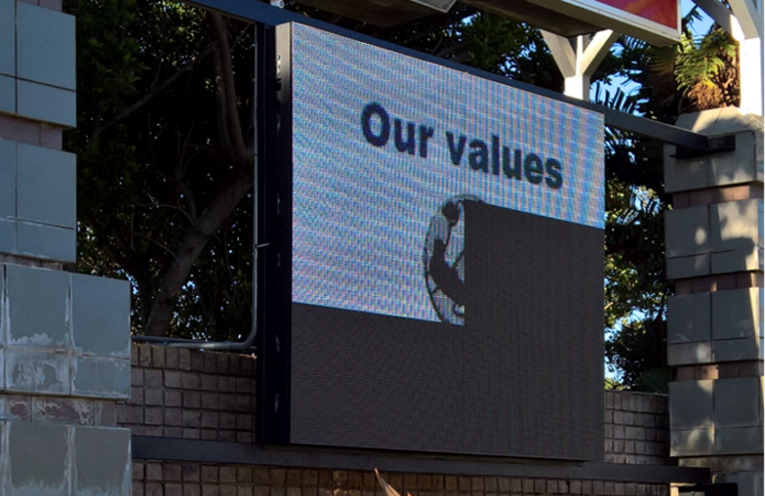
\includegraphics[width=8cm]{broken.png}
\caption{Een LED-display met verbindingsproblemen}
\end{figure}

Smart LEDs kunnen een oplossing bieden voor deze problemen. Elke LED beschikt namelijk over zijn eigen microcontroller. Dit verwijdert de nood aan verbinding met een grid aangezien de besturing bij de LED zelf gebeurd. Hierdoor krijgen de LEDs meer bewegingsvrijheid en wordt het makkelijker om delen van het display te vervangen. Daarbij beperken storingen ten gevolge van controllerproblemen zich tot slechts 1 LED waardoor reparaties aan het display beperkter zijn.  Verder kunnen SmartLEDs samen werken door met elkaar te communiceren. Dit gebeurt via VLC (\textit{Visual Ligth Communication}) waarbij visueel licht gebruikt wordt om informatie door te zenden\cite{VLC}. Hiervoor gebruiken ze hun ingebouwde LED die zowel als zender als als ontvanger kan dienen. 


\section{Verwant werk}
Dit project is een rechtstreeks vervolg op het project van vorig jaar waarin de SmartLEDs ontwikkeld werden. 

Daarnaast is er al veel onderzoek gebeurd rond LEDs en hun mogelijk tot signaaloverdracht. Zo werd er al door ETH Zurich en Disney research onderzoek gedaan naar de mogelijkheden van VLC networks waarbij verschillende microcontrollers met elkaar communiceerden via LEDs\cite{VLCNetworks}.


\section{Evaluatie}

Het doel van ons onderzoek is nagaan of een display opgebouwd uit SmartLEDs een meerwaarde biedt ten opzichte van gewone displays. We gaan na welke problemen opduiken en onderzoeken hier oplossingen voor.

Onze belangrijkste criteria zijn de flexibiliteit van het display en de mogelijkheid tot interactie met het display. Met flexibiliteit bedoelen we dat het mogelijk moet zijn om de SmartLEDs te verplaatsen zonder dat hiervoor code moet worden aangepast. Dit betekent dat de communicatie met en door de SmartLEDs onafhankelijk moeten werken van hun positie in het display. 

Voor de interactie willen we dat deze op een betrouwbare en interactieve manier gebeurt. Hiervoor maken we gebruik van een "lichtpen". Dit is een SmartLED voorzien van enkele knoppen om zo input door te sturen naar het display. Aan de hand van een floodlight, een lichtpen voorzien van meerdere, krachtigere LEDs, kunnen grotere groepen SmartLEDs aangestuurd worden.


\section{Implementatie}
Om onze hypothese te testen maakten we gebruik van LEDs verbonden met Zigduino r2 microcontrollers. We maakten gebruik van infrarood LEDs voor de communicatie om extra licht flikkeringen in het display te voorkomen en om interferentie van de omgeving zo veel mogelijk te vermijden.


\section{Oplossing}

\subsection{Onderlinge communicatie}
Om een vlak display te bekomen, moeten de LEDs uiteraard zijdelings staan. Dit zorgde helaas voor problemen, aangezien elke LED een specifieke invalshoek heeft. Wij hadden echter geen LEDs met een hoek van 180\degree ter beschikking. Als oplossing probeerden we een diffuser te gebruiken maar hierdoor verzwakte het licht van onze LEDs waardoor er geen signaal kon worden verzonden. Mogelijk zou dit geen probleem zijn bij sterkere LEDs maar deze zouden problemen kunnen geven omdat ze teveel energie vragen. 

Met twee naar elkaar gerichte LEDs lukt het ons wel om een bit-string door te zenden. Deze opstelling bestaat uit een eerste LED die een bit-string uitzendt, een tweede die deze ontvangt en doorgeeft aan een microcontroller en vervolgens een derde die de ontvangen bit-string weer uitzendt in een andere richting. In minder conventionele LED-displays (met een vorm die het toelaat de LEDs naar een elkaar te richten of met bewegende onderdelen) is onderlinge communicatie dus wel mogelijk.

\subsection{Meerdere LEDs}
Bij aanvang van ons project hoopten we voor het display en het verzenden van informatie dezelfde LED te gebruiken. Dit is niet alleen compacter dan met meerdere LEDs maar het zorgt er ook voor dat we de SmartLED niet moeten uitbreiden met extra hardware. Helaas bracht dit extra moeilijkheden met zich mee, zoals informatie die verzonden moest worden over een LED die volgens het display geen licht mag uitzenden. Ook maakte dit onze code veel complexer en  

Om deze redenen kozen we om met een tweede LED te werken. Ook besloten we om de communicatie via een infrarood LED te laten verlopen, zo vermijden we dat de communicatie-LEDs signalen zouden opvangen van de display-LEDs. Bovendien creëert dit meer mogelijkheden voor het display aangezien het volledige RGB spectrum kan gebruikt worden om afbeeldingen weer te geven. 

\subsection{Externe lichtbron}
Omdat een tweede LED ook een externe lichtbron is, valt uit het voorgaande al te besluiten dat een goed gericht licht in staat is om te interageren met een SmartLED-display. 

Wij onderzochten twee manieren waarop interactie met het LED-display mogelijk was. Dit aan de hand van een lichtpen (een LED met een microcontroller achter) die op een bepaalde manier geprogrammeerd was.

De eerste manier bestond uit een reactie van het display wanneer een signaal verzonden werd, versus wanneer er geen verzonden werd. We programmeerden hiervoor een soort "\textit{Whack-a-mole}" spel waarbij de speler een bepaalde tijd heeft om te reageren op een licht verandering door de lichtpen hierover te laten schijnen. Zowel bij succes als bij mislukking geeft het display feedback door weer van licht te veranderen (zie figuur \ref{fig:mole}).
\begin{figure}
\centering
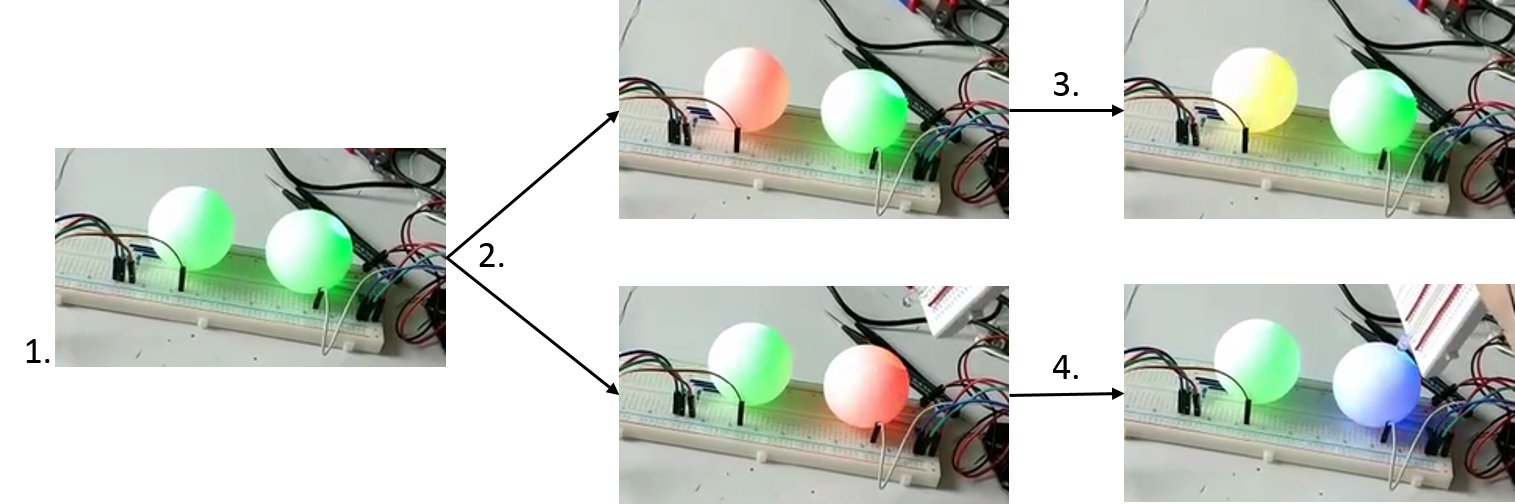
\includegraphics[width=8cm]{moleSequence.png}
\caption{1:inactief, 2:vraagt om respons, 3:geen respons, \mbox{4: wel respons}}
\label{fig:mole}
\end{figure}

Bij de tweede manier wordt er een bit-string verzonden naar het display. Deze manier hebben we getest met een programma waarbij een bit-string gelijk werd gesteld aan een kleur die de display LED moest aannemen of aan een programma dat afgespeeld moest worden.

\subsection{Omgevingslicht}
Om ervoor te zorgen dat de SmartLEDs een verschil zien tussen omgevingslicht en een signaal, moeten we een threshold instellen. Om ervoor te zorgen dat onze code niet afgesteld was op 1 plaats, maakten we deze dynamisch. Op bepaalde tijdstippen in ons programma wordt een meting genomen om de hoeveelheid omgevingslicht vast te stellen. Als threshold wordt dan een iets hogere waarde genomen zodat omgevingslicht niet en een signaal (feller licht) wel over de grens komt.

\begin{figure}
\centering
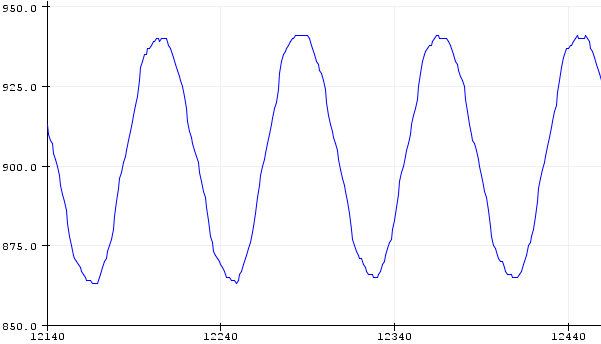
\includegraphics[width=8cm]{ruis.png}
\caption{De gedetecteerde ruis, gemeten spanning in functie van de tijd}
\label{fig:ruis}
\end{figure}

We merkten op dat deze threshold niet hetzelfde bleef voor eenzelfde hoeveelheid omgevingslicht. Bij het visualiseren van de spanning was te zien dat de gedecteerde ruis sinusoïdaal verloopt (zie figuur \ref{fig:ruis}). Dit valt te verklaren door de RC-kringen in de gebruikte zigduino's. Om de gemeten waarde van het omgevingslicht nauwkeuriger te maken besloten we om deze gelijk te stellen aan het gemiddelde van een tiental metingen met telkens 50ms (ongeveer de helft van een periode) tussen om het sinusoïdale verloop op te vangen. Hierbij tellen we opnieuw een waarde op, vergelijkbaar met de amplitude van de sinus golf, en bekomen zo onze threshold. Dit proces wordt weer meerdere keren herhaald doorheen de uitvoering van het programma.


\section{Conclusie}
We concluderen dat SmartLED-displays geen alternatief zijn voor conventionele LED-displays maar dat ze toch over bepaalde eigenschappen beschikken die ze niet alleen bruikbaar maar ook bijzonder maken. Ze kunnen interactief gebruikt worden als simpele, vlakke displays zonder onderlinge communicatie maar ook zonder eventuele verbindingsproblemen. Daarnaast kunnen ze in andere vormen wel signalen doorgeven en dus meer als 1 geheel functioneren.


\section{Verder werk}
Als vervolg op dit project zou een display opgebouwd uit echte SmartLEDs gemaakt kunnen worden. Het zou ook interessant zijn mocht er een oplossing gevonden worden voor het probleem met de invalshoek van de LEDs zodat zijdelings gecommuniceerd kan worden.


\bibliographystyle{named}
\bibliography{bronnen}

\end{document}

